%tout ce qui est dans ce chapitre doit etre succint%
%l'approfondissement se fera dans la seconde partie avec%
%le cas d'étude%

\chapter{Qu'est ce que l'Intelligence Artificielle ?}
%definition du terme intelligence, intelligence artificelle%
%diagramme cercle avec IA, machine learning et deep learning%
%pour faire comprendre que le AI > ML > DL% 
\begin{figure}[!h]
    \centering
    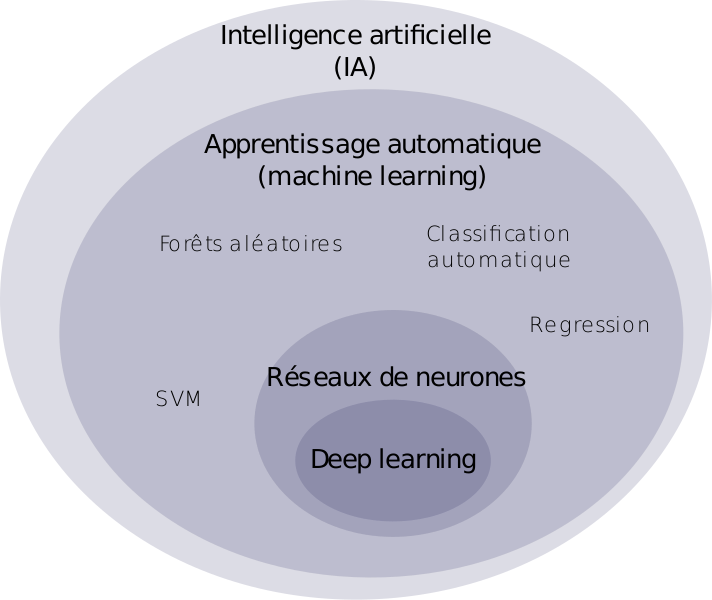
\includegraphics[width=0.8\textwidth]{Images/aitype}
\end{figure}

\section{Machine Learning}
%trouver des illustration pour facilité la compréhension%
%donner de simple exemple concret% 


\section{Deep Learning}
%trouver des illustrations aussi%
%trouver des exemples: Deepmind, watson etc%
Le deep learning est un subset du machine learning, 

\chapter{}